\newline
%\newline
\section{Background}\label{sec:background}
\subsection{Sequential Prefetching}
There are several implementations of prefetchers. The simplest form can be achieved with a sequential prefetcher\cite{prefetching}. These prefetchers tries to keep the cache pre-loaded with the data that is needed for the next instructions by fetching the next block upon a cache-miss. An improved version of the sequential prefetcher is the tagged sequential prefetcher. This adds an extra \emph{tag} to the cache blocks, and if there is a hit on a set tag, the prefetcher will fetch the next block.

\subsection{Reference Prediction Tables}
RPT prefetching involves the use of a large table to keep track of missed load instructions that have previously been called. 
\begin{figure}[!htb]
    \centering
    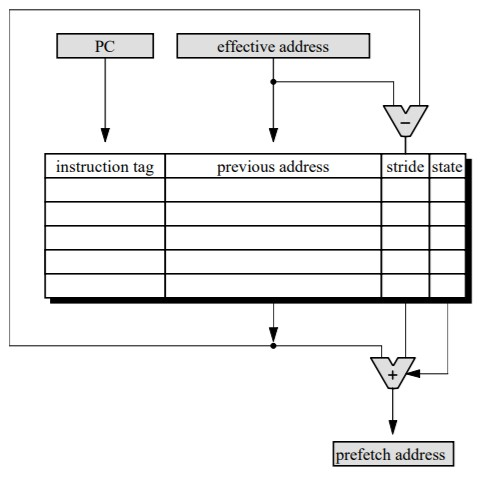
\includegraphics[width = 7cm]{images/RPTable.jpg}
    \caption{Organization of the Reference Prediction Table\cite{RPTimage}.}
    \label{fig:RPT Layout}
\end{figure}
Figure \ref{fig:RPT Layout} describes the layout of each table line. Each time a data block is missed, the address is stored in the ``Last Address'' field of the and the state is set to initial. The next time this data load results in a miss, the ``Last Address" is subtracted from the current address and the difference is stored in the ``Delta" field, and the state is now set to training. The third time this instruction results in a miss, the new delta is calculated, if the deltas are a match, the state is set to confirmed, and there is now a strided access pattern. The prefetcher can now load the next block into the cache prior to that load instruction being executed. 


\subsection{Program Counter/Delta-Correlation}
In the PC/DC method of prefetching, a Global History Buffer (GHB) is utilized to keep track of any cache hits or misses \cite{PCDC}. Figure \ref{fig:GHB Layout} describes how a GHB is structured.
\begin{figure}[!htb]
    \centering
    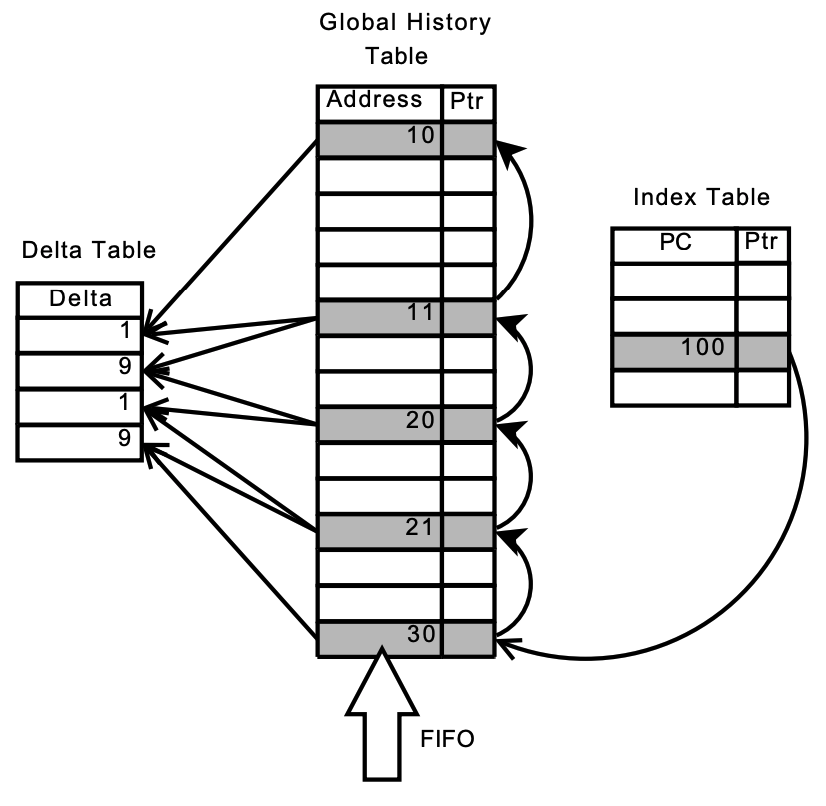
\includegraphics[width = 7cm]{images/GHBexample.png}
    \caption{Global History Buffer\cite{Book}.}
    \label{fig:GHB Layout}
\end{figure}
 Each time there is a miss, the index table will record the address of the respective block, and a pointer will be stored that points to the most recent miss from the same instruction. Each entry in the GHB also contains a pointer that references the next miss issued by the same instruction. Because we now have a ``chain" of pointers, we can traverse each one to see the pattern of the deltas between each address requested by each instruction that results in a miss. Now, the prefetcher will calculate said deltas, and store the values in the delta table. By traversing the stream of deltas, a pattern may be found. Once a pattern is detected, the prefetcher can start using the pattern to prefetch the predicted blocks.
 
%% State of the art subsection
\subsection{State of the Art} \label{subsec:state-of-the-art}
The DCPT functions similarly by finding a delta, or stride, between commonly accessed blocks. The DCPT method uses a table, similar to RPT. The table is indexed by the program counter (PC) of the instruction issuing a load. Table \ref{tab:DCPT} is an example of how a DCPT entry may look like.

\begin{table}[!htb]
\centering
\caption{Delta-Correlating Prediction Table.}
\label{tab:DCPT}
\begin{tabular}{ |c|c|c|c|c|c| } 
    \hline
    PC & Last Addr & Last Prefetch & Delta 1 & Delta n & Delta Pointer
    \\
    \hline
\end{tabular}
\end{table}

The last address field functions the same as RPT. The delta fields are initialized to 0, and the delta pointer field points to the head of the delta buffer. When a load instruction yields another miss, the delta is calculated like before, if the delta is 0, the buffer is not updated. After the buffer is updated, it is then traversed in reverse order to find a match to the most recently stored pair of deltas. Once a match is be found, the prefetcher adds the delta value to the last address, and stores this in the last prefetch field and sends it to a temporary prefetch candidate buffer. This process is repeated for each of the deltas following the matched pair. If the new prefetch candidate matches the last prefetch field, the entire content of the buffer is discarded up to this point.
Once the candidate buffer is finished, each entry is checked to see if it is in cache or not. If it is not, it is checked against the miss status registers to see if the block has been recently requested. Then, the candidate is checked against another buffer holding other prefetch requests that have yet to be completed. If the buffer is not full, the last prefetch field can be updated with the address, and the prefetch can take place.





